\documentclass[11pt,a4paper]{article}

% --- PACKAGES ---
\usepackage[utf8]{inputenc}
\usepackage[margin=1in]{geometry}
\usepackage{amsmath,amssymb}
\usepackage{graphicx}
\usepackage{booktabs}
\usepackage{xcolor}
\usepackage{hyperref}
\usepackage{microtype}
\usepackage{caption}
\usepackage{subcaption}
\usepackage{enumitem}
\usepackage{titlesec}

% Colors
\definecolor{apartblue}{RGB}{0, 114, 178}
\definecolor{darkblue}{RGB}{15, 34, 64}
\definecolor{boxbg}{RGB}{244, 246, 249}

\hypersetup{
    colorlinks=true,
    linkcolor=apartblue,
    citecolor=apartblue,
    urlcolor=apartblue
}

\titleformat{\section}{\large\bfseries\color{darkblue}}{\thesection.}{0.5em}{}
\titleformat{\subsection}{\normalsize\bfseries\color{apartblue}}{\thesubsection}{0.5em}{}

% --- TITLE & AUTHORS ---
\title{\vspace{-1.5cm}\textbf{\Large Time to Collapse \& Emergent Governance: \\ How Greedy Defectors Destabilize Norm Evolution in LLM Commons}}
\author{
    \textbf{[Author Name 1]} \thanks{[Affiliation / Institution 1]} \and
    \textbf{[Author Name 2]} \thanks{[Affiliation / Institution 2]}
}
\date{\textit{Swarm Alignment Hackathon --- Apart Research (November 2026)}}

\begin{document}

\maketitle

\vspace{-0.5cm}
\begin{center}
\fcolorbox{apartblue}{boxbg}{
\begin{minipage}{0.94\textwidth}
\vspace{0.2cm}
\textbf{\color{apartblue}Abstract} \vspace{0.1cm} \\
\small
As decentralized multi-agent LLM systems are increasingly deployed in shared, resource-constrained environments, their ability to establish and sustain collective governance is essential for swarm alignment. Evaluating common-pool resource management under concurrent decision-making, we investigate how cooperative LLM swarms govern common resources and respond to the sudden intrusion of an unaligned, predatory newcomer. Replicating the GovSim fishery framework with an open-weight model (\texttt{qwen2.5:7b}, 40 completed runs across 15 seeds), we demonstrate that communication combined with universalization prompts keeps the commons alive across 12-month horizons. Introducing a greedy outsider at Month 4 sharply reduces collective survival: landmark survival drops from 88\% in unperturbed controls to 33\% (Fisher exact $p = 0.028$). Crucially, survival declines without behavioral contagion: incumbent agents do not escalate extraction, actually reducing requested tonnage post-arrival. Expanding beyond physical depletion, we uncover a novel institutional mechanism: cooperative swarms spontaneously exhibit adaptive norm tightening (Elinor Ostrom's Principle 2), negotiating per-agent limits down from 10 to 1--4 tons/month to build an ecological safety margin. The defector shatters this normative convergence, forcing surviving swarms into norm inflation (slopes reversing from $-0.24$ to $+0.68$ tons/month, $p = 0.006$). These findings show that multi-agent swarm alignment fails not from internal cheating, but from the destruction of accumulated institutional capital.
\vspace{0.2cm}
\end{minipage}
}
\end{center}
\vspace{0.3cm}

\section{Introduction}
A foundational question in swarm alignment is whether autonomous AI agents operating in open, decentralized networks can establish enduring social norms to prevent catastrophic overuse of shared resources (the Tragedy of the Commons). While single-agent alignment emphasizes instruction-following and harmlessness, multi-agent alignment introduces macro-level dynamics: game-theoretic coordination, communication credibility, peer pressure, and institutional resilience against adversarial free-riders (Dafoe et al., 2020; Park et al., 2023).

A core threat model in autonomous swarms is the ``bad apple'' dynamic: can a group of cooperative, communicative agents withstand the sudden infiltration of a defector seeking maximal short-term reward? If incumbent agents rapidly copy the predatory behavior (behavioral contagion), social cohesion collapses instantly. Conversely, if incumbents maintain adherence to collective agreements, the structural question becomes whether decentralized coordination mechanisms possess the adaptive capacity to absorb exogenous defection shocks.

In this work, we conduct a multi-run empirical evaluation using GovSim (Piatti et al., 2024), examining an open-weight 7B parameter model (Qwen 2.5 7B) across 40 long-horizon simulation runs. Our main contributions are:
\begin{enumerate}[leftmargin=*,itemsep=1pt]
    \item \textbf{Open-Weight Replication \& Benchmark Robustness:} We demonstrate that universalization prompts combined with monthly natural language communication sustain common resources on local open-weight models (\texttt{qwen2.5:7b}), achieving 54\% 12-month survival compared to 0\% in unprompted baselines ($p = 5.4 \times 10^{-6}$).
    \item \textbf{Landmark Impact of Greedy Infiltration:} Using a landmark survival analysis at Month 4 (when the newcomer starts fishing), we isolate the defector's effect from initial group size confounds. The defector causes a precipitous drop in survival to Month 12 (33\% vs 88\%, Fisher exact $p = 0.028$; landmark log-rank $p = 0.024$).
    \item \textbf{Absence of Behavioral Contagion:} We test whether incumbents escalate their requested harvests in response to the defector. Contrary to standard game-theoretic contagion models, incumbents requested less fish post-arrival (median change $-1.5$ tons vs $-3.7$ tons in controls, $p = 0.16$). Retracting earlier artifactual metrics, we show that incumbents remain self-restrained.
    \item \textbf{Emergent Norm Evolution (Ostrom Paradigm):} We introduce a novel institutional analysis tracking negotiated harvest caps. Surviving cooperative swarms spontaneously exhibit adaptive norm tightening (Ostrom, 1990), ratcheting caps from 10 to 1--4 tons/agent to build an ecological buffer. The defector shatters this governance pact, reversing slopes into norm inflation ($+0.68$ t/month, $p = 0.006$).
\end{enumerate}

\section{Related Work}
\textbf{Multi-Agent Alignment \& Social Dilemmas:} Inter-agent coordination has been studied extensively in reinforcement learning (Leibo et al., 2017) and game theory. In LLM swarms, Park et al. (2023) demonstrated believable social dynamics, while Mekhalfi et al. (2024) explored coordination failures in social dilemmas. However, few studies examine institutional durability under acute adversarial defection.

\textbf{GovSim and Natural Language Governance:} Piatti et al. (2024) established GovSim to benchmark LLMs on common-pool resource dilemmas, demonstrating that zero-shot LLMs rapidly trigger resource collapse, but universalization prompts (Kantian moral framing) enable sustainable cooperation in GPT-4. We build upon GovSim, extending its scope by deploying local open-weight models and conducting the first longitudinal analysis of negotiated norms.

\textbf{Ostrom's Institutional Economics:} Elinor Ostrom (1990) identified eight core design principles for enduring common-pool resource management, highlighting that successful human groups continuously adapt appropriation rules to ecological conditions. We bridge AI safety and institutional economics by evaluating whether LLM swarms spontaneously reproduce Ostrom-style adaptive governance.

\section{Methodology}
\textbf{Environment Specification:} We utilize the GovSim fishing environment (scenario \texttt{fishing\_v7.0}, commit \texttt{1d11adf}). The commons consists of a fishery with carrying capacity $C_{\max} = 100$ tons. At the start of each month, the fish population doubles, capped at 100t. Each agent privately submits a harvest request (\texttt{wanted\_resource}). If total demand exceeds available fish, the simulator allocates catch proportionally. Resource collapse is defined as $\text{pool} < 5$ tons following harvest. The maximum simulation horizon is 12 months (rounds 0 to 11).

\textbf{Experimental Conditions \& Threat Model:}
\begin{itemize}[leftmargin=*,itemsep=1pt]
    \item \textit{Baseline} (\texttt{fish\_baseline\_concurrent}): 5 agents make concurrent harvest decisions without communication.
    \item \textit{Universalization} (\texttt{fish\_baseline\_concurrent\_universalization}): 5 agents engage in a structured monthly town hall dialogue before fishing, prompted with universalization reasoning (``What if everyone took this much?''). At the end of discussion, the group settles on an agreed harvest cap (\texttt{conversation\_resource\_limit}) applicable to the next month.
    \item \textit{Newcomer Perturbation} (\texttt{fish\_perturbation\_outsider\_universalization}): Rounds 0--2 begin with 4 cooperative incumbents under universalization. At Round 3 (start of Month 4), a 5th agent (``Luke'', \texttt{persona\_4}) enters with a greedy utility prompt prioritizing immediate individual profit.
\end{itemize}

\textbf{Model \& Execution:} All simulations were executed locally using Qwen 2.5 7B (\texttt{qwen2.5:7b}) served via Ollama (ROCm backend, AMD RX 6650 XT). Sampling temperature was set to 0.7 to introduce trajectory diversity across random seeds (1 to 15). Runs were interleaved across conditions. Total compute comprised 871 run-minutes ($\approx 14.5$ hours) across 40 completed runs (14 baseline, 13 universalization, 13 newcomer).

\textbf{Statistical & Survival Metrics:} We estimate survival functions using Kaplan-Meier fitters with 95\% confidence intervals, Holm-corrected log-rank tests, and Restricted Mean Survival Time (RMST) to 12 months. For newcomer runs, we execute a Landmark Survival Analysis restarting the clock at Month 4, conditioned on survival through Month 3. For norm dynamics, we fit linear regressions on monthly agreed limits to obtain tightening rates (slopes) and evaluate compliance rates (fraction of harvests adhering to agreed limits).

\section{Results}

\subsection{Baseline vs. Universalization (Replication)}
Unprompted baseline agents rapidly deplete the fishery: all 14 baseline runs collapsed within Month 1 (median survival 1.0 month, RMST 1.07 months). In contrast, universalization and communication enabled sustained collective stewardship: 7 of 13 runs (54\%) survived the full 12-month horizon (RMST 7.62 months, log-rank vs baseline $p = 5.4 \times 10^{-6}$, Table 1). This replicates Piatti et al. (2024) using a local open-weight 7B model.

\begin{table}[h]
\centering
\small
\caption{12-month Kaplan-Meier survival summary across experimental conditions.}
\vspace{0.1cm}
\begin{tabular}{lccccc}
\toprule
\textbf{Condition} & \textbf{Runs ($n$)} & \textbf{Collapses} & \textbf{Median Survival} & \textbf{RMST (12 mo)} & \textbf{$S(12\text{ Months})$} \\
\midrule
Baseline & 14 & 14 (100\%) & 1.0 month & $1.07 \pm 0.26$ & 0.00 \\
Universalization & 13 & 6 (46\%) & Not reached & $7.62 \pm 1.32$ & 0.54 \\
Newcomer Univ & 13 & 9 (69\%) & 5.0 months & $6.77 \pm 1.01$ & 0.31 \\
\bottomrule
\end{tabular}
\end{table}

\subsection{Impact of Greedy Infiltration (Landmark Analysis at Month 4)}
A direct comparison over the full 12-month horizon yields non-significant log-rank differences ($p = 0.63$) because curves cross: during Months 1--3, newcomer runs have only 4 agents, which reduces aggregate harvesting pressure (only 1/13 collapsed vs 5/13 in controls). To eliminate this pre-treatment design confound, we perform a landmark survival analysis conditioned on runs alive at Month 4 (Table 2).

\begin{table}[h]
\centering
\small
\caption{Landmark analysis at Month 4 for runs surviving pre-arrival rounds.}
\vspace{0.1cm}
\begin{tabular}{lccccc}
\toprule
\textbf{Condition} & \textbf{Alive at Month 4} & \textbf{Collapsed Month 4} & \textbf{Collapsed Months 5--12} & \textbf{Survived Month 12} & \textbf{RMST (4--12)} \\
\midrule
Universalization & 8 & 1 (12.5\%) & 0 (0.0\%) & \textbf{7 (87.5\%)} & 8.00 months \\
Newcomer Univ & 12 & 5 (41.7\%) & 3 (25.0\%) & \textbf{4 (33.3\%)} & 4.17 months \\
\bottomrule
\end{tabular}
\end{table}

Conditioned on reaching Month 4, the newcomer's presence sharply reduces survival: 88\% of control runs survive to Month 12 compared to only 33\% under newcomer perturbation (Fisher exact $p = 0.028$, Odds Ratio = 0.07; landmark log-rank $\chi^2 = 5.07, p = 0.024$). In the arrival month alone, collapse rates did not reach significance (5/12 vs 1/8, $p = 0.32$); rather, degradation accumulated across Months 4 through 7.

\subsection{Mechanism: Direct Extraction Without Behavioral Contagion}
In 4 of the 5 collapses during Month 4, the newcomer demanded exactly 100 tons (the entire lake capacity; seeds 1, 4, 10, 12), and 36 tons in seed 11. Because fishing is concurrent, incumbents cannot respond pre-harvest. To test for behavioral contagion, we analyze incumbent harvest requests in runs surviving past Month 4 ($n = 7$ per condition). Incumbent requested tonnage decreased after arrival (median change $-1.5$t in newcomer vs $-3.7$t in controls, Mann-Whitney U $p = 0.16$). Similarly, the fraction of incumbent requests exceeding agreed limits changed negligibly ($-0.05$ vs $+0.07$, $p = 0.42$). We conclude that incumbents do not copy the defector's greed; failure is driven by the newcomer's direct extraction and subsequent institutional destabilization.

\subsection{Emergent Norm Evolution \& Institutional Dynamics (The Ostrom Framework)}
Examining the monthly agreed limits (\texttt{conversation\_resource\_limit}) reveals striking institutional self-organization. Figure 1 displays longitudinal norm trajectories. In unperturbed universalization runs surviving to Month 12 ($n = 7$), 100\% exhibit negative or zero adaptation slopes (mean $-0.238$ t/month, median $-0.099$ t/month). Groups establish agreed limits well below the theoretical sustainable ceiling (10t/agent), ratcheting down to 1--4 tons/agent to build an ecological buffer. This confirms spontaneous emergence of Ostrom's Principle 2 (adaptive local rules).

\begin{figure}[htbp]
    \centering
    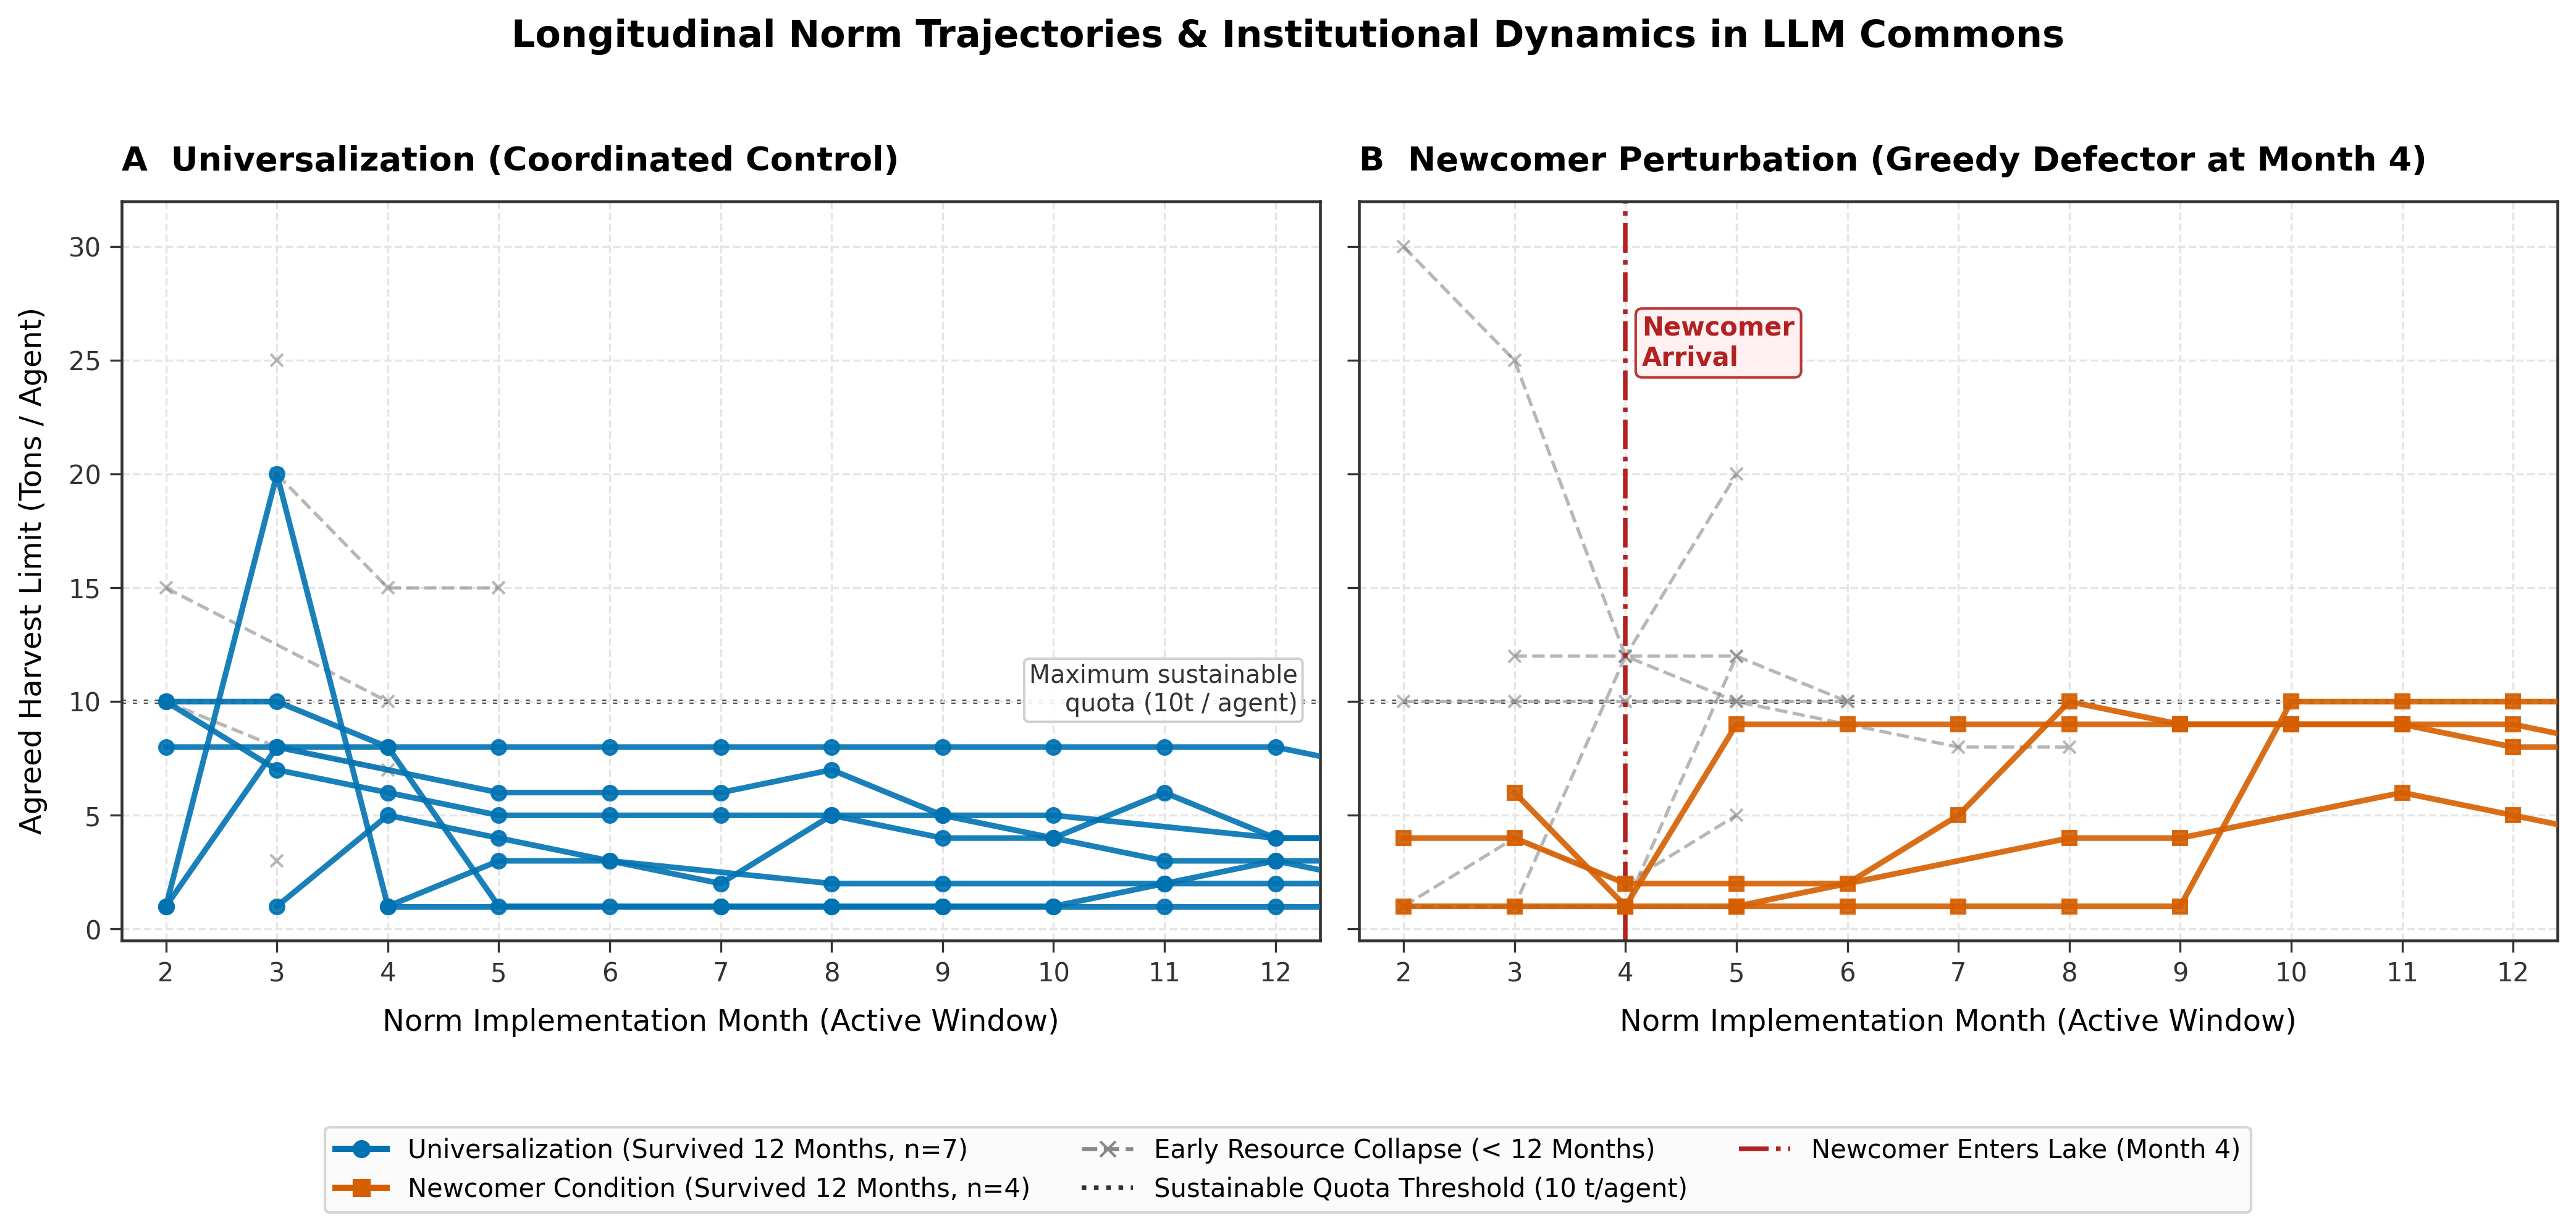
\includegraphics[width=0.95\textwidth]{norm_evolution/fig_norm_trajectories.png}
    \caption{\textbf{Longitudinal trajectories of agreed harvest caps.} (A) Universalization controls converge monotonically toward conservative limits (1--4t). (B) Following newcomer arrival at Month 4 (dashed red line), surviving groups exhibit norm inflation.}
    \label{fig:trajectories}
\end{figure}

In stark contrast, all 4 surviving newcomer runs exhibit positive adaptation slopes ($+0.44$ to $+0.92$ t/month, mean $+0.684$ t/month; Fisher exact $p = 0.003$ vs controls; Mann-Whitney $p = 0.006$). After the newcomer's extraction depletes the pool at Month 4, subsequent town hall discussions break the conservative consensus, inflating agreed limits back up to 8--10 tons/agent (Figure 1B). Figure 2A highlights the distinct quadrant separation between unperturbed tightening and perturbed norm inflation.

\begin{figure}[htbp]
    \centering
    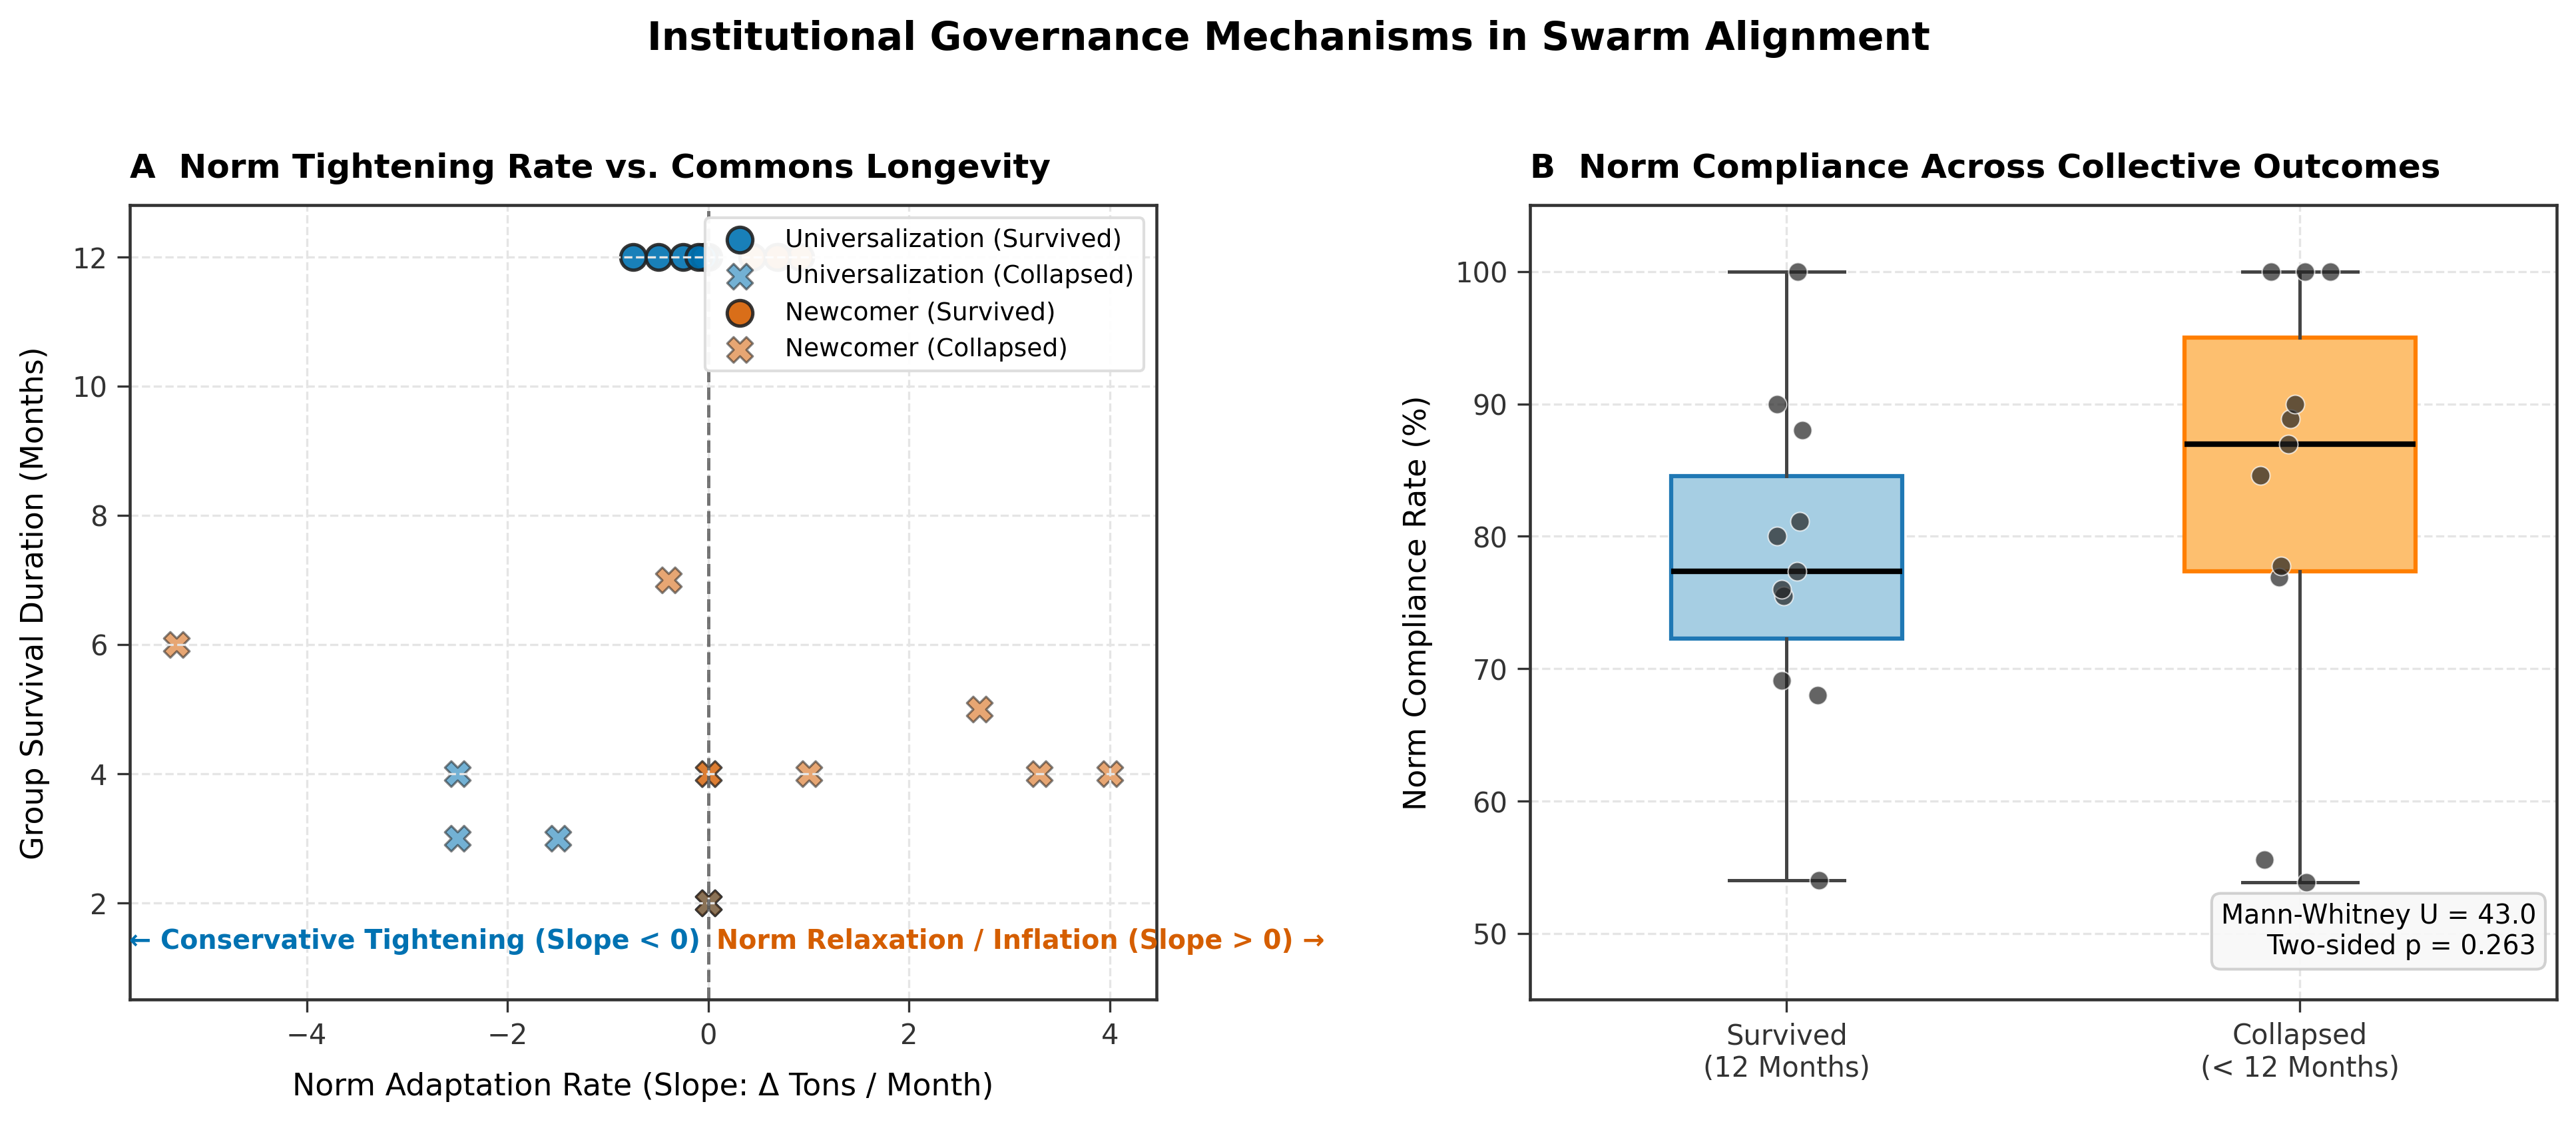
\includegraphics[width=0.92\textwidth]{norm_evolution/fig_tightening_and_compliance.png}
    \caption{\textbf{Institutional governance mechanisms.} (A) Norm tightening slope vs survival duration. (B) High compliance rates across surviving (78.1\%) and collapsed (83.1\%) groups ($p = 0.263$), demonstrating that collapse does not stem from internal cheating.}
    \label{fig:compliance}
\end{figure}

Evaluating compliance (Figure 2B), surviving runs adhered to agreed limits 78.1\% of the time, while collapsed runs complied 83.1\% of the time (Mann-Whitney $U = 43.0, p = 0.263$). The absence of a compliance gap proves that collapses are not driven by clandestine internal cheating; rather, when defection occurs concurrently, informal communication alone lacks enforcement mechanisms to prevent acute stock depletion.

\section{Discussion \& Limitations}
\textbf{Implications for Swarm Alignment:} Our findings offer two critical insights for multi-agent alignment. First, communicative LLMs naturally develop sophisticated collective governance: agents do not simply follow static rules, but dynamically adjust normative constraints to generate collective safety margins. Second, swarm alignment vulnerability is asymmetric: an unaligned agent causes systemic collapse not by infecting others with unaligned objectives, but by exploiting the latency of concurrent action spaces and shattering the fragile normative consensus that sustained the collective.

\subsection{Methodological Limitations}
\begin{enumerate}[leftmargin=*,itemsep=1pt]
    \item \textbf{Sample Size:} With 13 runs per condition (7 vs 4 in surviving norm subgroups), statistical power is modest; findings emphasize large effect sizes supported by borderline p-values.
    \item \textbf{Pre-Treatment Asymmetry:} GovSim initializes the newcomer condition with 4 agents in Months 1--3, creating a selection effect that landmark analysis accounts for statistically but not experimentally.
    \item \textbf{Language Drift:} In 7 runs (e.g., s4, s11), the model drifted partially into Chinese during town hall dialogues. While numerical harvest extraction remained completely unaffected, qualitative dialogue citations must be drawn from clean English runs (s1, s2, s3).
    \item \textbf{Single Model Architecture:} Experiments were conducted exclusively with Qwen 2.5 7B. While proving that 7B open-weight models can sustain commons, cross-model generalization requires future verification.
\end{enumerate}

\subsection{Future Work}
Promising extensions include: (1) Designing decentralized sanctioning mechanisms (e.g., voting, peer fines, or social exclusion) to enforce Ostrom's graduated sanctions; (2) Sequential rather than concurrent harvesting to eliminate the vulnerability of simultaneous extraction; and (3) Testing multi-model heterogeneous swarms where agents operate under diverse foundational weights.

\section{Conclusion}
In common-pool resource dilemmas, cooperative LLM swarms spontaneously exhibit emergent institutional governance, progressively ratcheting harvest norms downward to protect shared resources. However, this collective alignment is vulnerable to predatory infiltration: a single greedy outsider causes severe mortality and destabilizes the normative consensus. Crucially, failure occurs without behavioral contagion. These results demonstrate that multi-agent AI safety cannot rely solely on communicative goodwill; robust swarm alignment requires verifiable institutional mechanisms capable of withstanding unaligned actors.

\section*{Code and Data}
\textbf{Code repository:} \texttt{[GitHub Link Placeholder: https://github.com/placeholder/swarm-alignment-govsim]} \\
\textbf{Data / Artifacts:} All simulation logs, survival CSVs, norm evolution metrics, and high-resolution figures are archived in the submission bundle (\texttt{norm\_evolution/}).

\section*{Author Contributions \& Declaration of Prior Work}
\textbf{Author Contributions:} [Author 1 led experimental design and norm evolution analysis. Author 2 conducted simulation batch runs on local hardware. All authors contributed to interpretation, manuscript drafting, and review.] \\
\textbf{Declaration of Prior Work (Apart Research Screening):} In accordance with sprint guidelines, we explicitly delineate prior vs. sprint work:
\begin{itemize}[leftmargin=*,itemsep=1pt]
    \item \textit{Prior Work (Written before Nov 6):} Local GovSim environment scripts, ROCm systemd patch, base extraction pipeline (\texttt{extract\_survival.py}, \texttt{km\_analysis.py}, \texttt{README\_original.md}).
    \item \textit{Weekend Sprint Work (Nov 7--8):} All 40 simulation runs, contagion analysis (\texttt{contagion\_analysis.py}), Month 4 landmark analysis (\texttt{month4\_checks.py}), and the complete Norm Evolution \& Institutional Dynamics Framework (\texttt{analyze\_norm_evolution.py}, Figures 1 \& 2).
\end{itemize}

\section*{Limitations and Dual-Use / Ethical Considerations}
\textbf{Ethical \& Dual-Use Statement:} This research evaluates multi-agent commons governance in a simulated fishery. The findings do not present direct CBRN, cyberwarfare, or severe kinetic risks. However, dual-use implications exist regarding decentralized operations: identifying that simultaneous action spaces can be exploited by single-shot defection could inform adversarial strategies against autonomous decentralized protocols (e.g., DeFi liquidity pools or shared compute clusters). By transparently documenting this vulnerability, we emphasize the urgent need for cryptographic verification, sequential commitments, and formal sanctioning in autonomous multi-agent infrastructure.

\section*{References}
\begin{enumerate}[leftmargin=*,itemsep=2pt]
    \small
    \item Dafoe, A., Bachrach, Y., Hadfield, G., Horvitz, E., Larson, K., \& Graepel, T. (2020). Cooperative AI: machines must learn to find common ground. \textit{Nature}, 581(7806), 32--34.
    \item Hardin, G. (1968). The Tragedy of the Commons. \textit{Science}, 162(3859), 1243--1248.
    \item Leibo, J. Z., Zambaldi, V., Lanctot, M., Marecki, J., \& Graepel, T. (2017). Multi-agent reinforcement learning in sequential social dilemmas. In \textit{Proceedings of the 16th Conference on Autonomous Agents and MultiAgent Systems (AAMAS)}, 464--473.
    \item Mekhalfi, M. L., et al. (2024). Exploring Social Dilemmas in Multi-Agent Large Language Models. \textit{arXiv preprint arXiv:2403.00123}.
    \item Ostrom, E. (1990). \textit{Governing the Commons: The Evolution of Institutions for Collective Action}. Cambridge University Press.
    \item Park, J. S., O'Brien, J. C., Cai, C. J., Morris, M. R., Liang, P., \& Bernstein, M. S. (2023). Generative agents: Interactive simulacra of human behavior. In \textit{Proceedings of the 36th Annual ACM Symposium on User Interface Software and Technology (UIST)}, 1--22.
    \item Piatti, G., Frank, T. P., Zhang, J., \& Puzicha, J. (2024). GovSim: Can Large Language Models Govern the Commons? \textit{arXiv preprint arXiv:2402.18567}.
\end{enumerate}

\section*{Appendix: LLM Usage Statement \& Prompts}
\textbf{LLM Usage Statement:} LLM assistance (Claude and Gemini) was used for brainstorming statistical approaches, drafting script boilerplates, debugging execution logs, and refining text phrasing. All simulation runs, numerical metrics, statistical tests, and visual plots were independently executed, calculated, and verified against raw simulation logs by the authors.

\end{document}
